O método utilizado para obtenção dos valores de Micro \textit{F1 Score} e acurácia para o \textit{Ensemble} foi o mesmo utilizado para os modelos de Rede Convolucional e \textit{Xtreme Gradient Boosting}. Ressaltando que os resultados das medidas de desempenho obtiveram os mesmos valores, sendo este o motivo de serem apresentados somente o valor da medida Micro \textit{F1 Score}. Na Tabela \ref{tbl:fscore} observa-se os resultados para cada modelo de Rede Convolucional, juntamente do resultado do \textit{Ensemble}.

\begin{table}[!htb]
\centering
\caption{F1 Micro das Arquiteturas utilizadas}
\label{tbl:fscore}
\begin{tabular}{@{}cc@{}}
\toprule
Modelo & F1 Micro           \\ \midrule
1      & 0.6898857620507105 \\
2      & 0.6767901922541097 \\
3      & 0.6606297018668152 \\
4      & 0.6798551128448036 \\
5      & 0.6667595430482028 \\
6      & 0.6781833379771524 \\
7      & 0.694901086653664  \\
8      & 0.6285873502368348 \\
9      & 0.6244079130677069 \\ 
ensemble & 0.7174700473669546 \\ \bottomrule
\end{tabular}
\end{table}

É observado que o melhor classificador, modelo 7, individual de CNN, obteve 69.49\% enquanto que o pior, modelo 9, obteve 62.44\%. Ressaltando que cada classificador de CNN usado no \emph{Ensemble} obteve resultados melhores do que os outros, em determinada expressão ou bons resultados em todas as expressões, mas não se sobressaiu em nenhuma expressão específica. No caso do modelo 9, obteve-se bons resultados em quase todas as expressões, mas nenhum resultado melhor na classificação de determinada expressão em relação aos outros modelos. Já no caso do modelo 7, obteve-se o melhor resultado de classificação para expressão de surpresa.

No modelo \textit{Ensemble} teve-se um total de 32.738.871 parâmetros treináveis, que é resultado da soma dos parâmetros treináveis dos modelos CNN, bem como do XGBoost. Onde o modelo de XGBoost possui uma quantidade pequena de parâmetros treináveis, em comparação com os modelos de CNN, pois, enquanto a quantidade deste está na ordem de milhares, os outros estão na ordem de milhões. Este comportamento se mostra coerente, se for levado em consideração as tarefas de cada modelo, que possuem complexidades bastante distintas.

Os modelos de CNN mais profundos, consequentemente com maior número de parâmetros treináveis, foram os que obtiveram melhores desempenho individuais.   Já os modelos mais rasos, apesar de obterem desempenho abaixo dos profundos, obtiveram os melhores resultados em classificar expressões específicas. Quantidade de parâmetros treináveis do \textit{Ensemble} podem ser visualizados na Tabela \ref{tbl:fscore}.

Na Figura \ref{fig:emsemble} é apresentado o resultado do modelo utilizando \emph{Ensemble}. Onde o resultado final de desempenho foi de 71.74\% de acordo com a métrica \emph{F1 Micro}, ressaltando que seu valor de Acurácia possui o mesmo valor. E com este resultado o \emph{Ensemble} supera, por pouco, o modelo campeão da competição.

\begin{figure}[!htb]
    \centering
    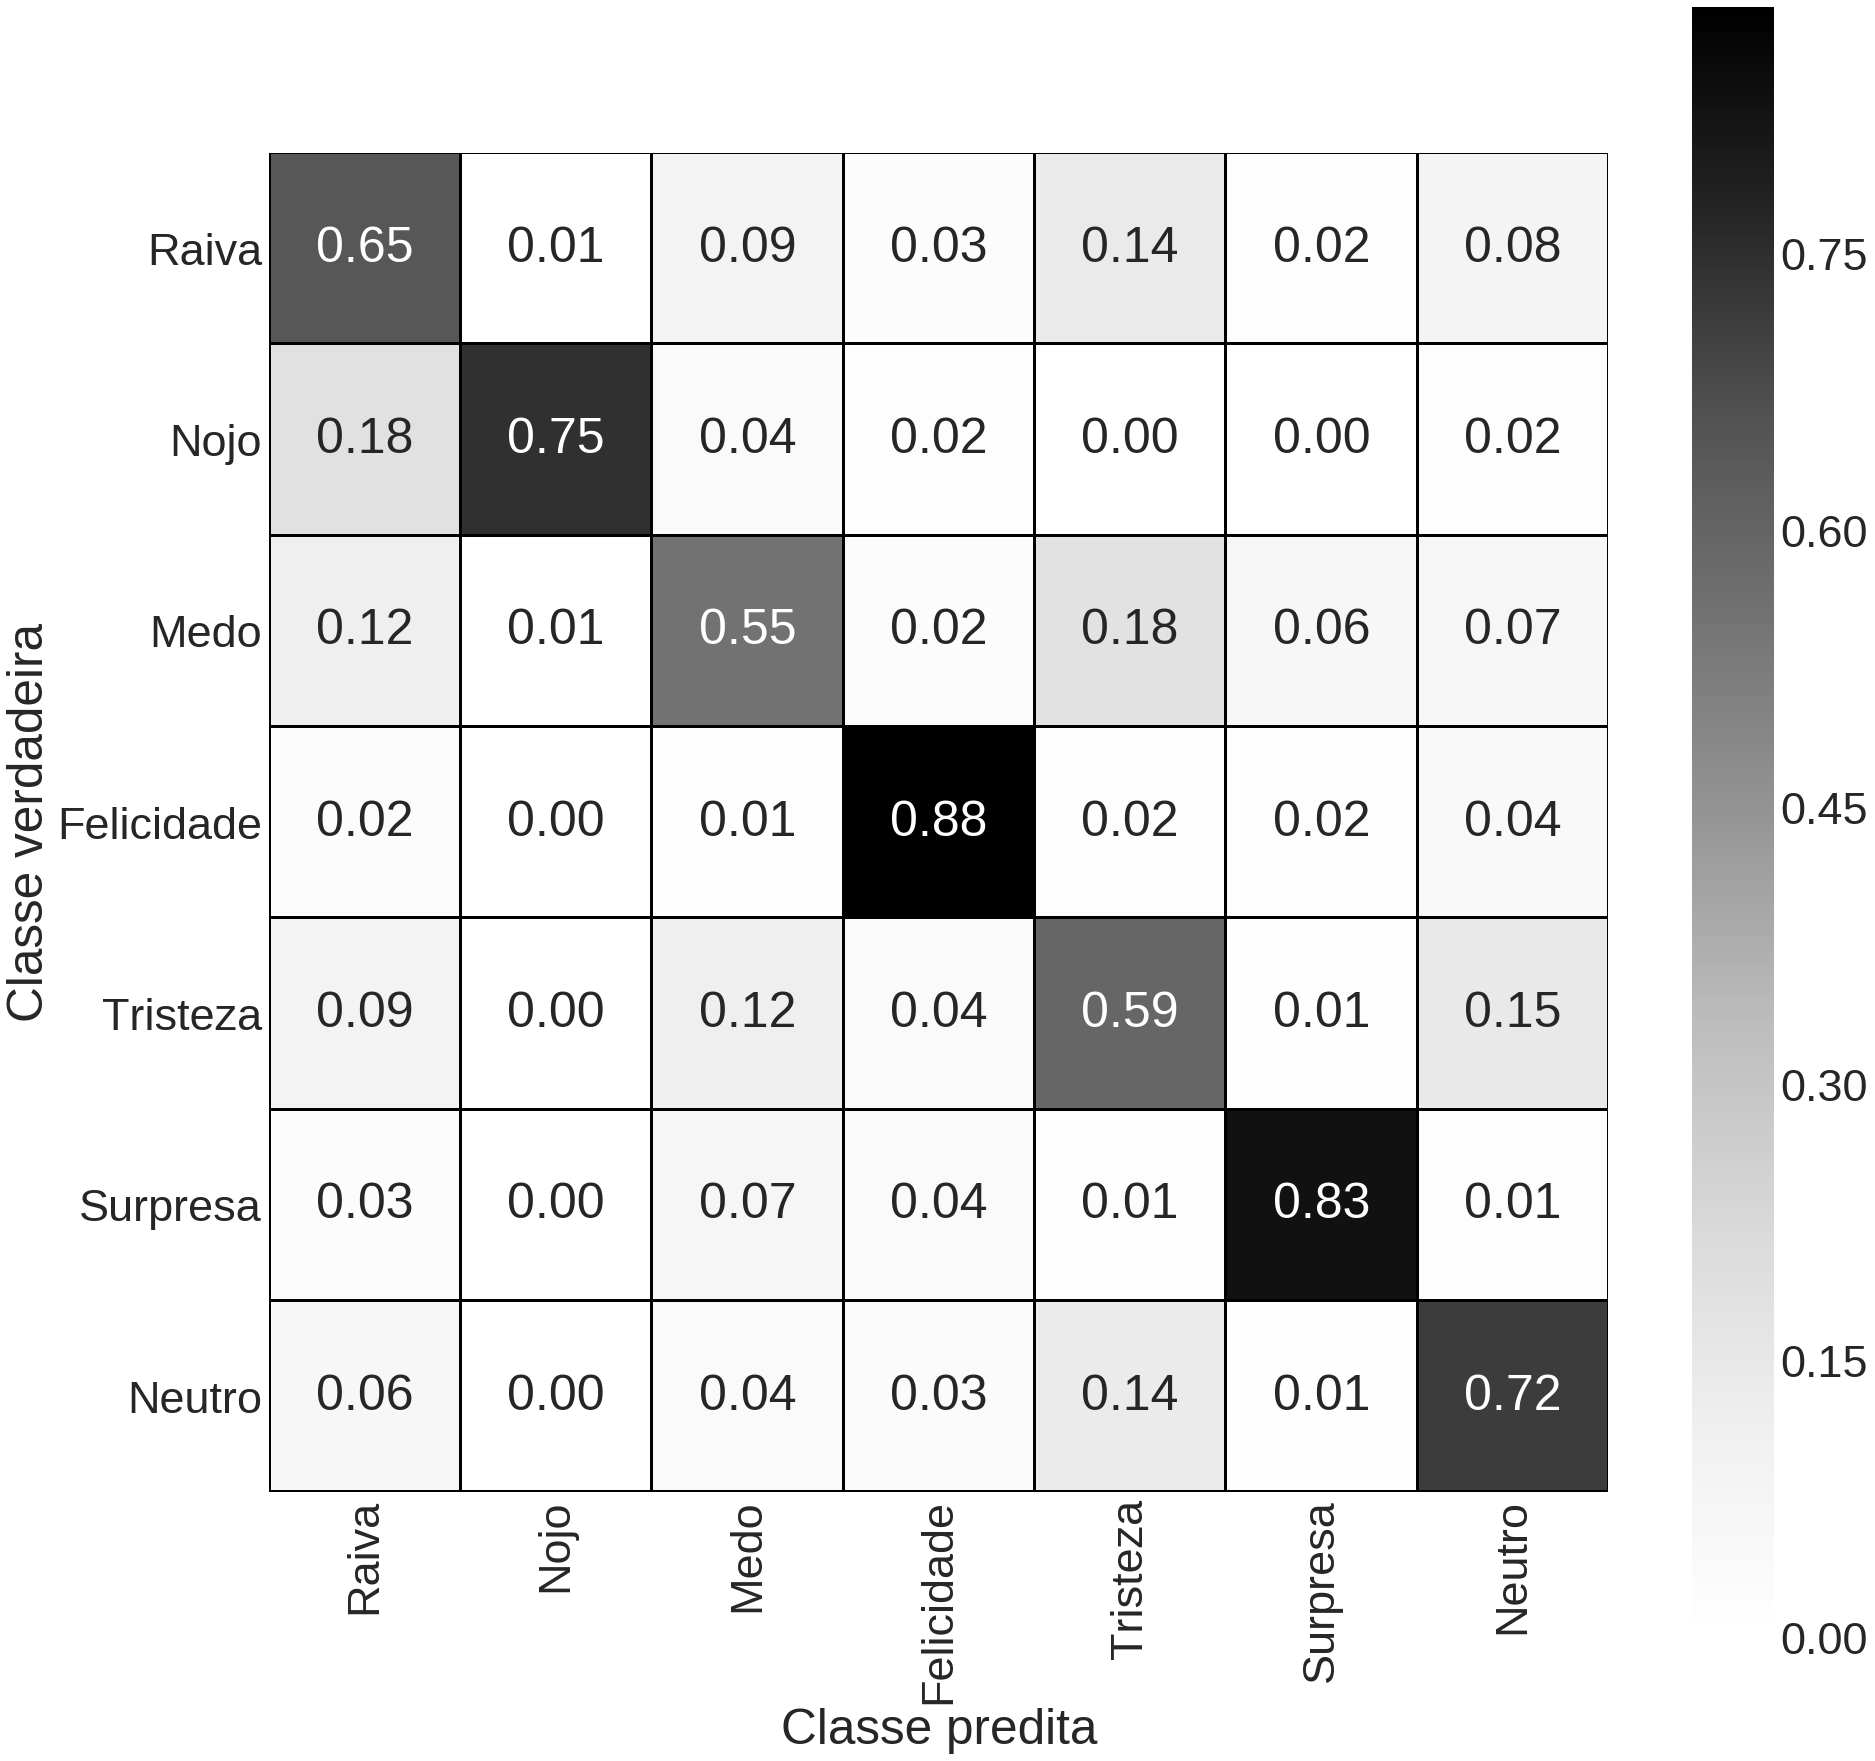
\includegraphics[width=9cm]{images/cm_emsemble.png}
    \caption{Matriz de Confusão do \emph{Ensemble} (CNN + \emph{XGBoost})}
    \label{fig:emsemble}
\end{figure}

Apesar do desbalanceamento da base de dados, a classificação da expressão de nojo obteve-se um dos melhores resultados \ref{fig:samples}, acompanhadas de surpresa e felicidade, com \textit{F1 Score} de
78\%, 83\%, e 89\% respectivamente. As classificações das outras expressões também apresentaram bons resultados, todas com \textit{F1 Score} maior ou igual a 58\%.

\begin{figure}[!htb]
    \centering
    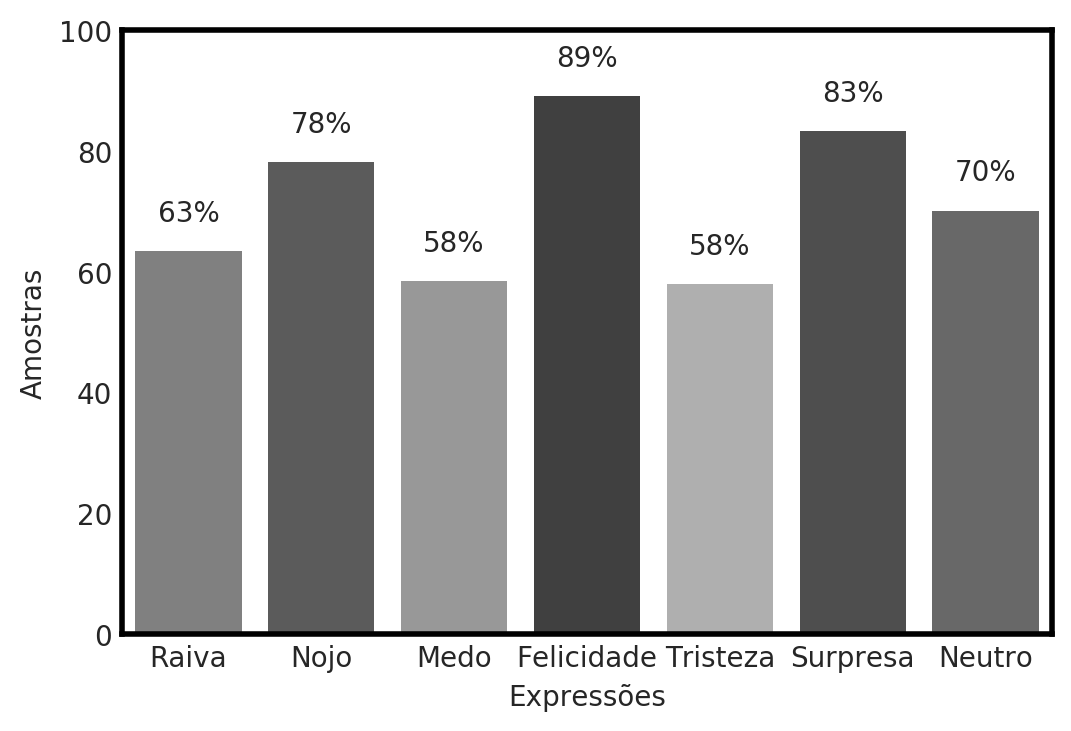
\includegraphics[width=8cm]{images/f1_bar.png}
    \caption{F1 Score por Expressão}
    \label{fig:f1_bar}
\end{figure}
